\chapter{Problem Motivation}

\section{Introduction}    

% Test single- and double-spacing around block quotes
The volume of scientific literature has doubled in the past 20 years\footnote{https://data.worldbank.org/indicator/IP.JRN.ARTC.SC}.  
The ubiquitous availability of computing and access to free, open-source software has also enabled exponential growth in publishing for fields like computer science.  
Figure \ref{figure1} shows a plot of the number of papers published on CS ArXiv\footnote{https://arxiv.org} each year 2015 to 2020 on a log scale. 

\begin{figure}[h]
    \centering
    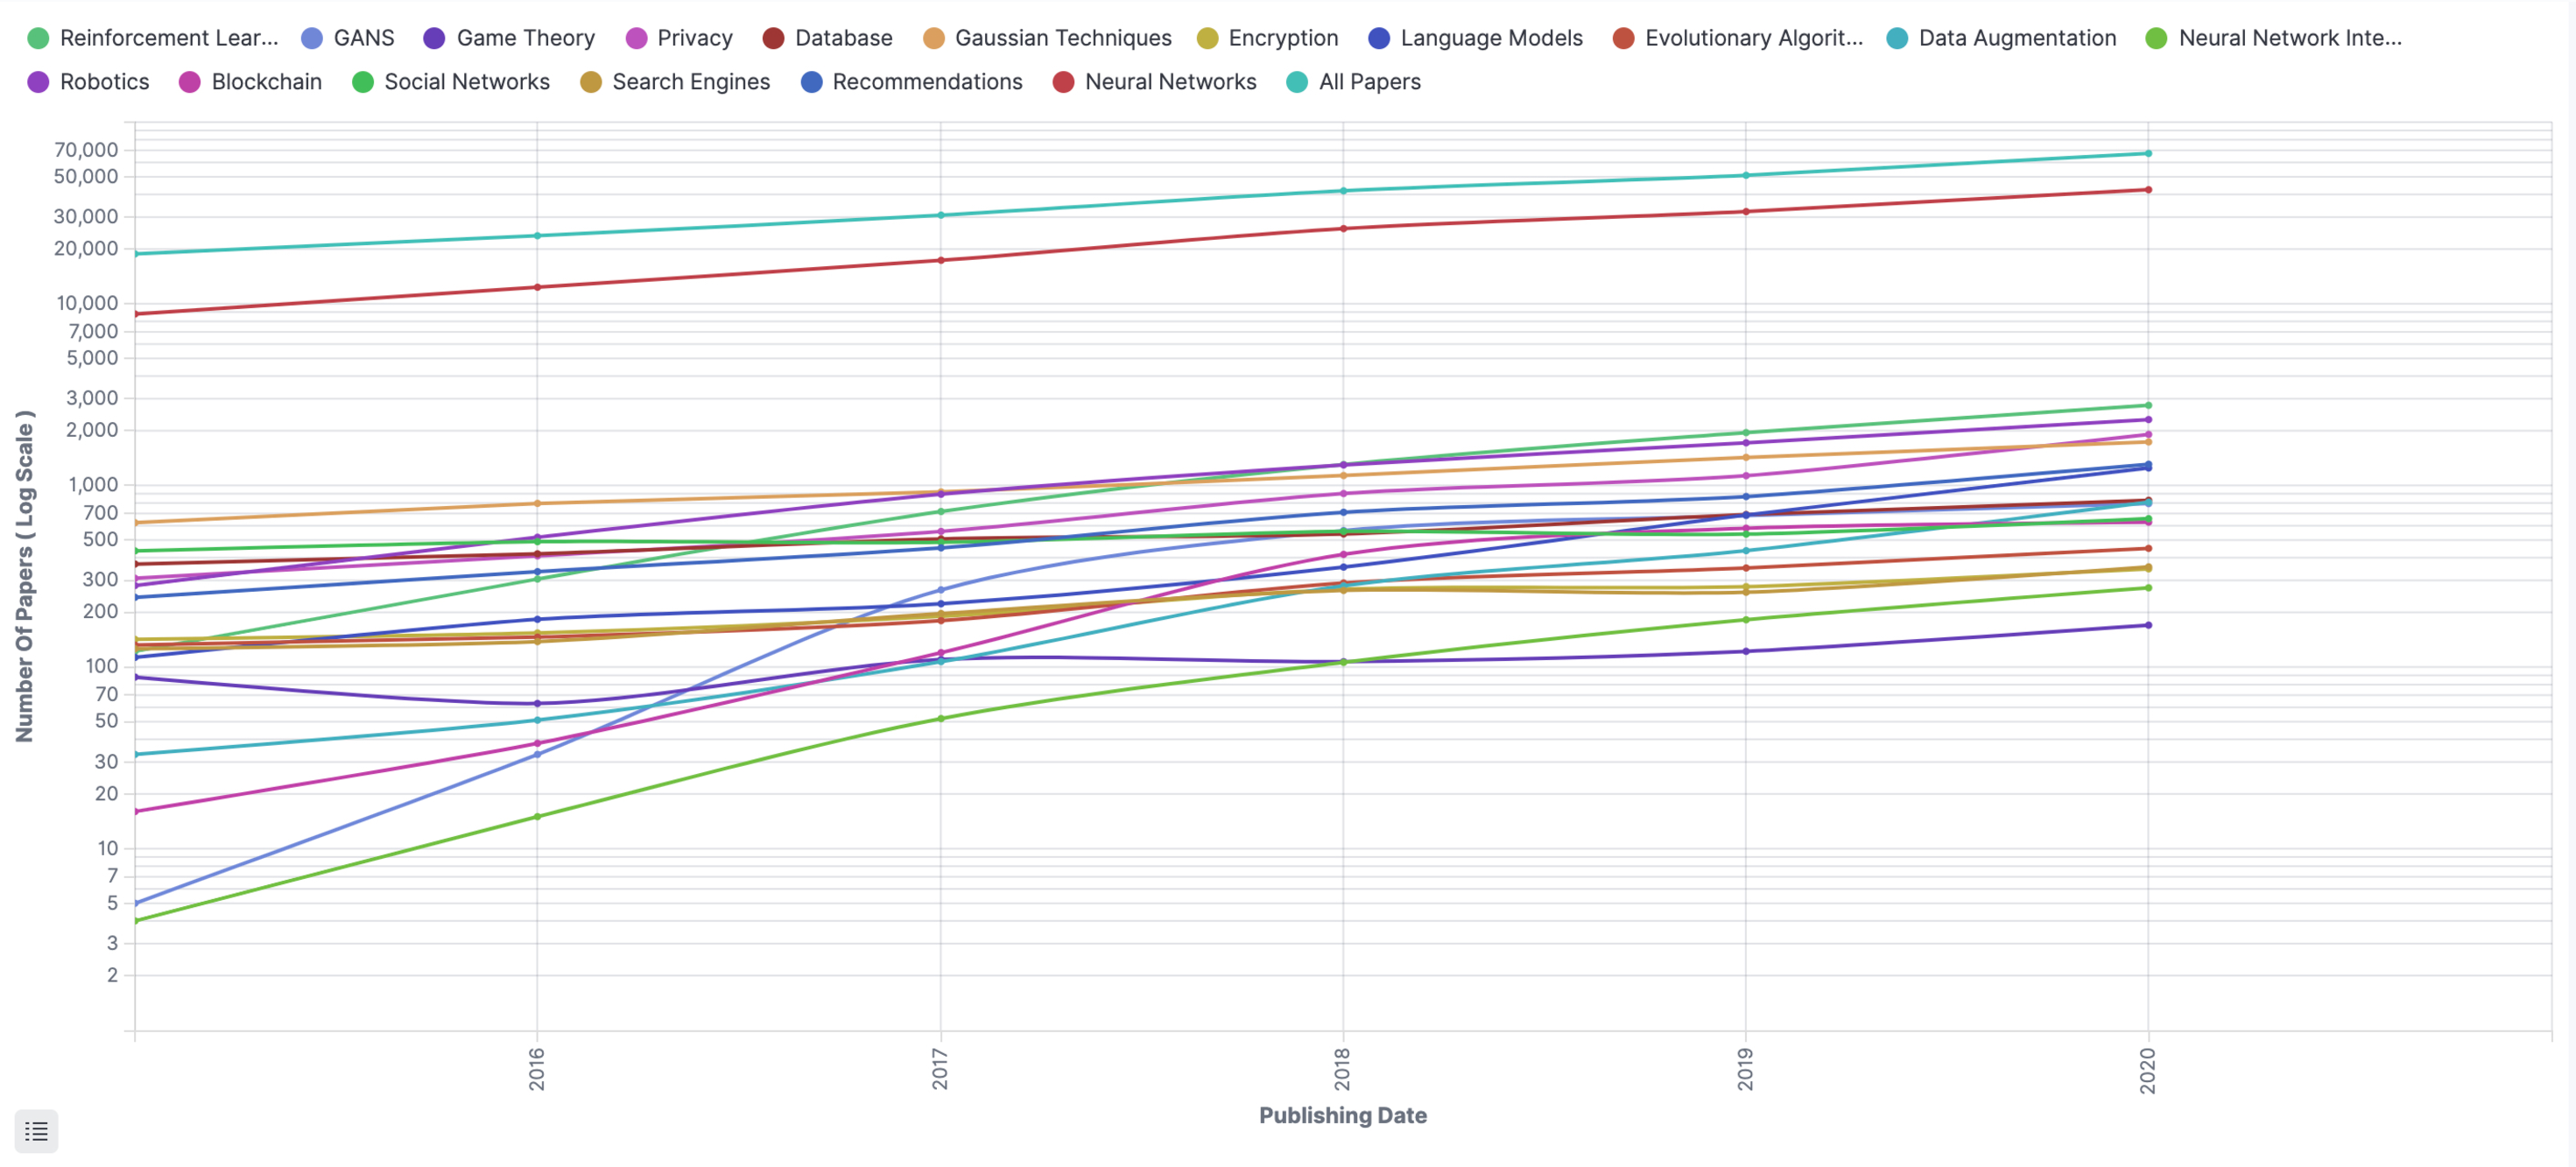
\includegraphics[width=\maxwidth{\textwidth}]{src/images/num-papers.pdf}
    \caption{ A time series plotting count of papers every year for across various topics in CS from January 2015 to December 2020}
    \label{figure\arabic{figurecounter}}
\end{figure}
\refstepcounter{figurecounter}

The growth in the volume of research has also led to academic research search engines becoming primary mediums of access for scientific literature. 
% \parencite{gusenbauer2020academic} showed that Google Scholar hosts more than 389M documents. 
Academic research search engines are different from traditional search engines like Google because they host content specific to scientific literature. 
Scientific papers generally undergos a process of peer-review. If a paper does not undergo peer-review it may still get cited by other publications/papers. This relational nature of academic research makes it fairly easy to filter credibility based on citations as a metric. Major academic research search engines such as Google Scholar, Microsoft Academic etc. leverage citations as a metric for ranking documents. Although citations are very useful, the increase in the number of documents can also result in a sea of noise for a particular search query. In such cases, the researcher gets minimal context information around search matches to infer more insight about why the document was surfaced. 

Researchers also tend to look for information which embedded deeper inside papers. Many papers contain some table of results for some experiments, Or some comparisons to techniques/methods from other papers. This type of tabular information is quite useful to get on the fly context about the results/comparsions being framed in a paper. Such information is generally not easily accessible through normal search engines. Platforms such as PapersWithCode\footnote{https://paperswithcode.com} host/track State-of-the-art leaderboards for ML along with thier papers. There are no currently available tools which augment  more context about a reasearch paper when reading research. 

% Generally reading through a research paper leads the researcher down citation trails, or makes the researcher look for information around the paper for further analysing and doing many such research oriented tasks which involve the understanding and analysis of scientific information. 

The next section aims to provide a motivating example to explain the lack of context in search results displayed by three large proprietary search engines.
% \textit{The next section will assess the “features” provided by these search engines to improve researcher productivity.}

\section{Motivating Example: Search Results From Academic Research Search Engines}
Machine Learning and deep learning research dominate the majority of CS publications on pre-print servers like ArXiv (Figure \ref{figure1}).
Taking that information into consideration, consider the use-case of a researcher trying to look for papers where a Transformer\parencite{vaswani2017attention} model written in PyTorch\parencite{paszke2019pytorch} is given adversarial examples. 
The researcher chooses to use the following search query: \textit{pytorch transformer adversarial examples} on the search engines Google Scholar, Semantic Scholar and Microsoft Academic. 
Ideally, the experiments of a paper or the appendix of a paper or the methodology section of a paper would consist of information about code/model in a paper. 
The following subsections will analyze the search results for this query for three large search engines: Google Scholar, Microsoft Academic and Semantic Scholar. 
\pagebreak
\subsection{Search Results From Google Scholar}
\label{sr-g}

\begin{figure}[h]
    \centering
    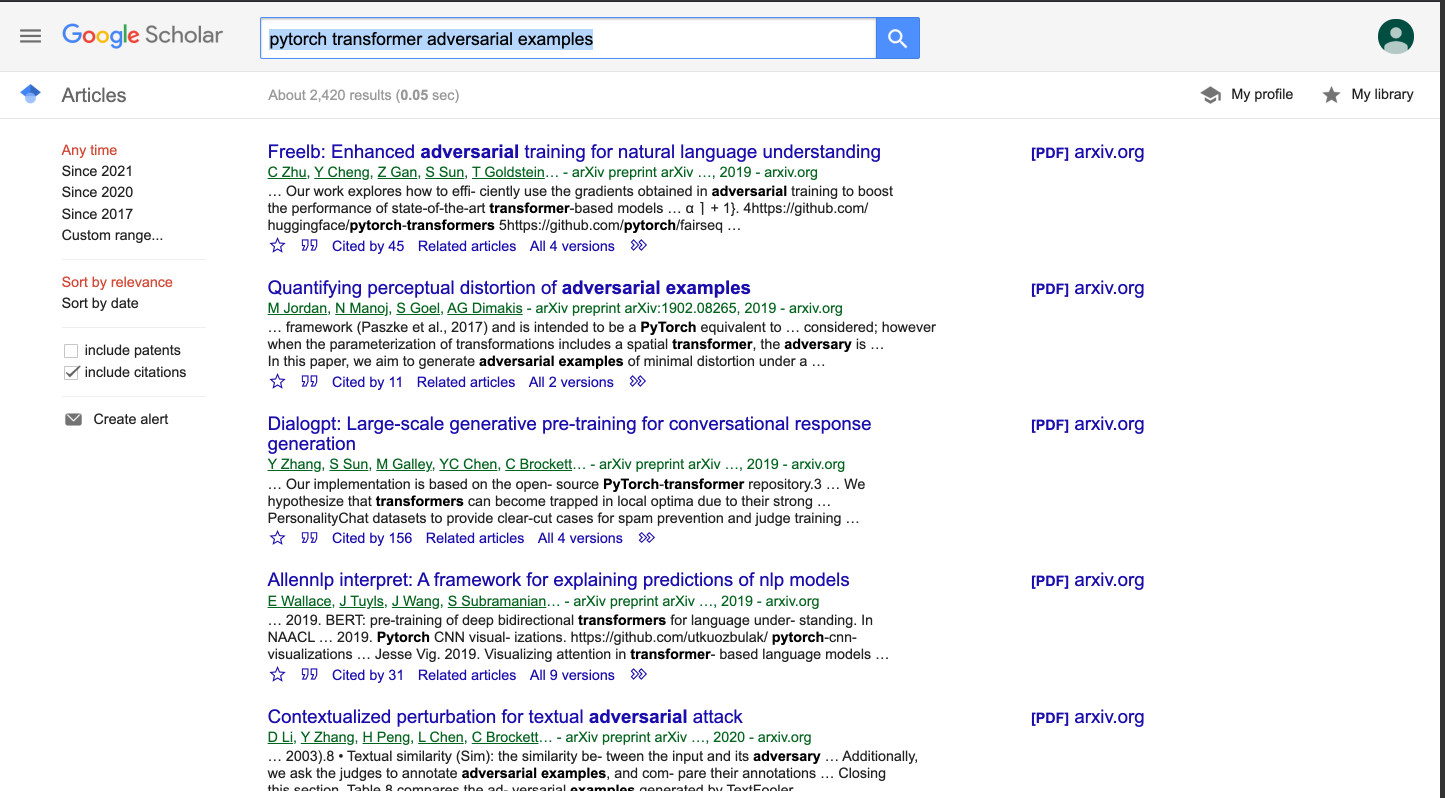
\includegraphics[width=\maxwidth{\textwidth}]{src/images/google-scholar-example.png}
    \caption{Search Results For Google Scholar}
    \label{figure\arabic{figurecounter}}
\end{figure}
\refstepcounter{figurecounter}
Although Google scholar found 2000+ search results, the search-result-fragments do not provide any additional context information about where the terms are matching. 
It highlights links to code-repositories but there is no mention of when and where those links were cited in the document. 

\pagebreak
\subsection{Search Results From Microsoft Academic}
\label{sr-m}
\begin{figure}[h]
    \centering
    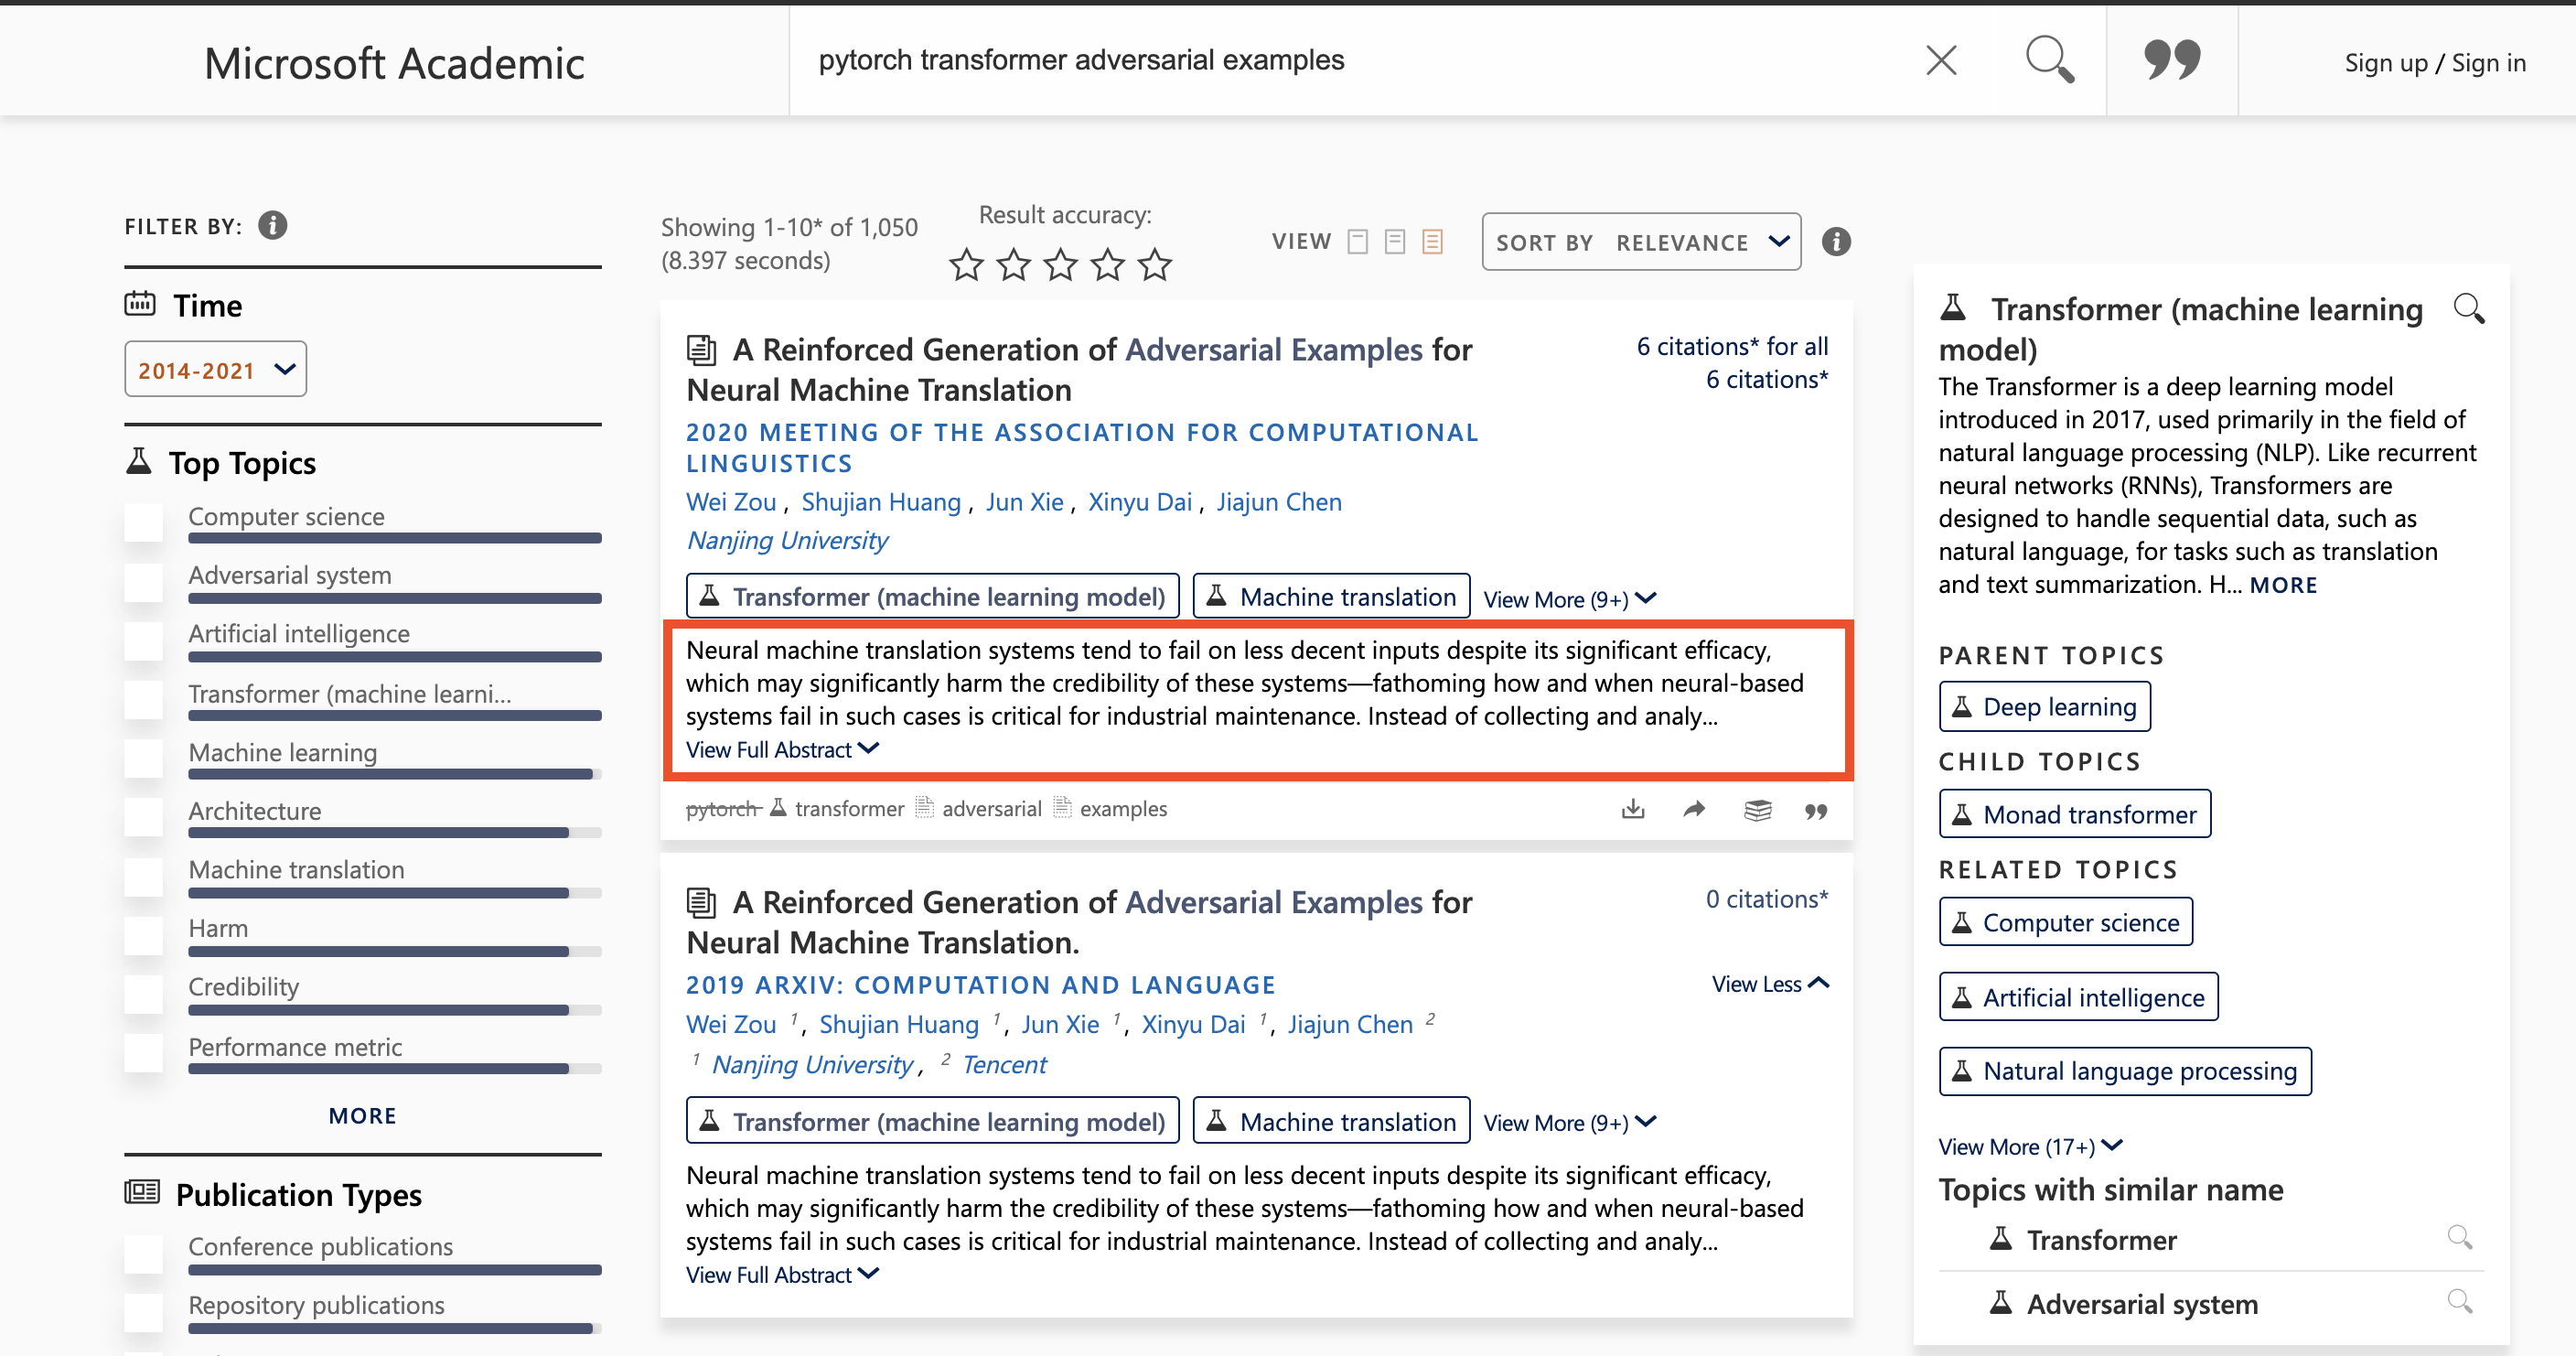
\includegraphics[width=\maxwidth{\textwidth}]{src/images/academic-example.png}
    \caption{Search Results For Microsoft Academic}
    \label{figure\arabic{figurecounter}}
\end{figure}
\refstepcounter{figurecounter}
Microsoft Academic provides additional information around context like topics, analytics on types of publication matches etc,
It fails to provide information about where the match has taken place in the paper.

\pagebreak
\subsection{Search Results From Semantic Scholar}
\label{sr-s}
\begin{figure}[h]
    \centering
    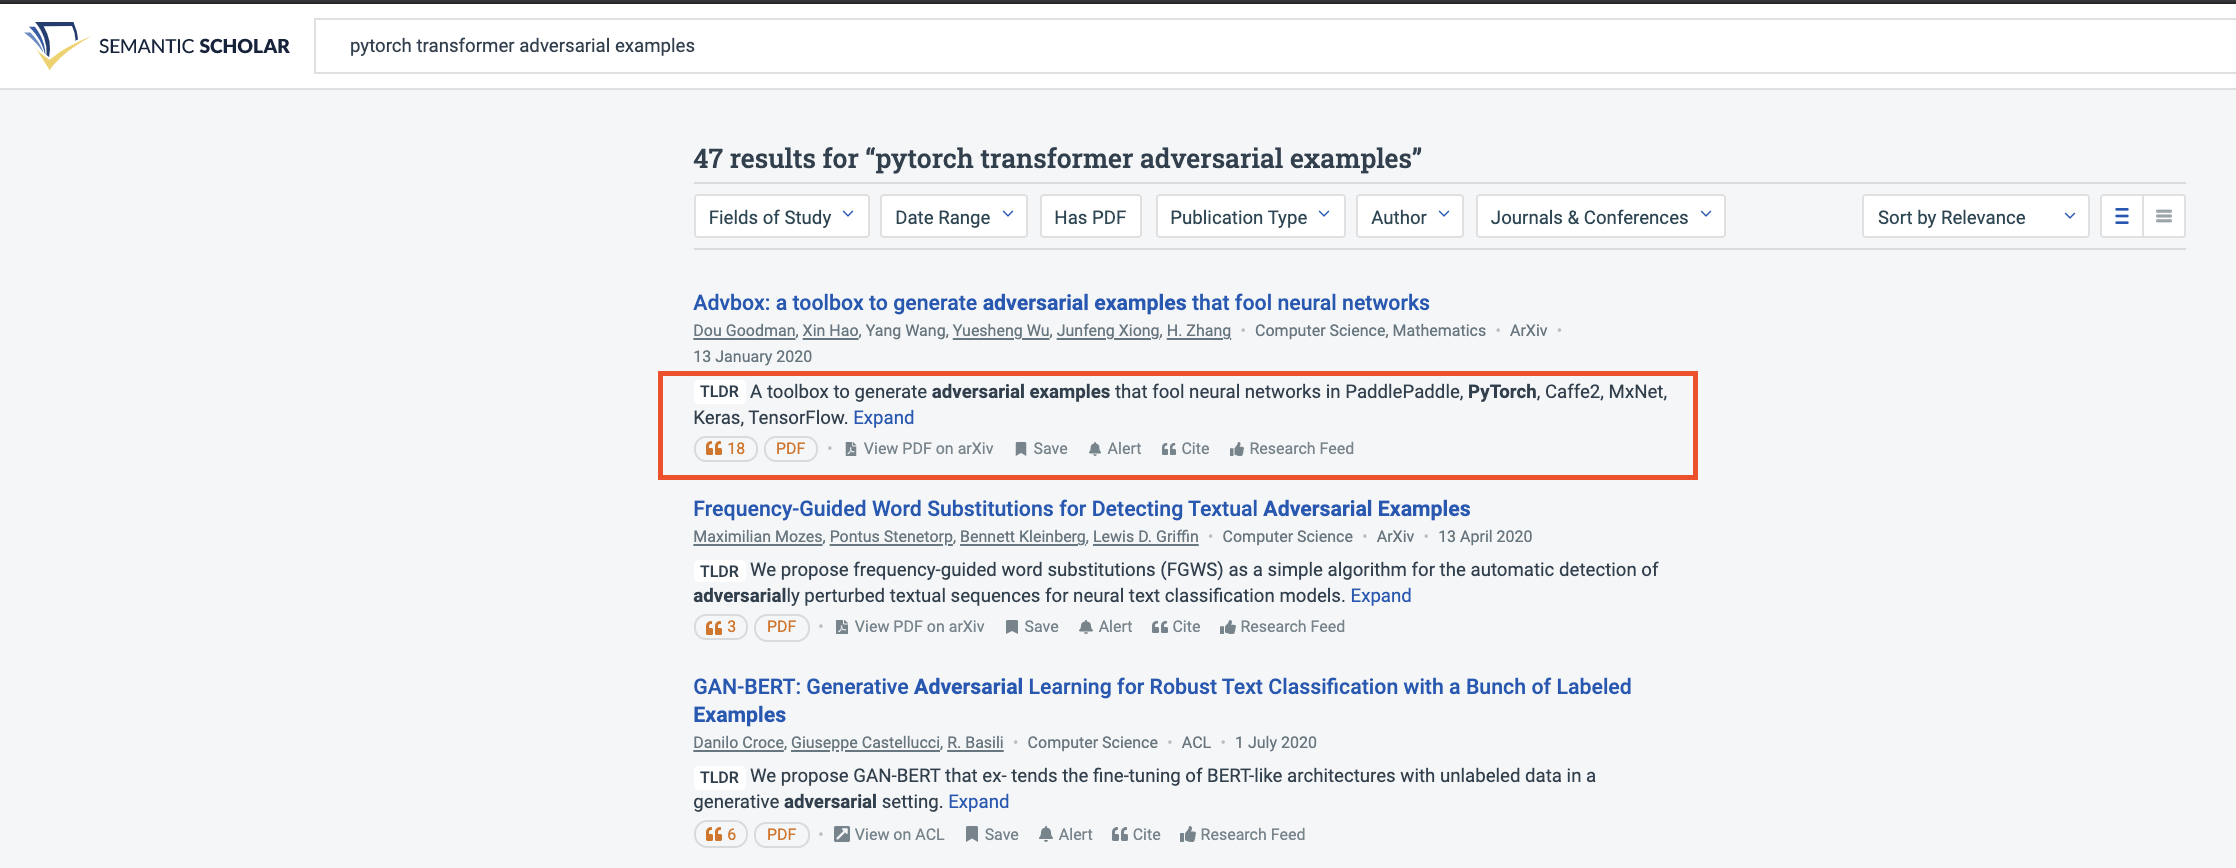
\includegraphics[width=\maxwidth{\textwidth}]{src/images/ss-example.png}
    \caption{Search Results For Semantic Scholar}
    \label{figure\arabic{figurecounter}}
\end{figure}
\refstepcounter{figurecounter}
Semantic Scholar highlights few search fragments where results would have matched and presents a smaller result set. 
But all search results do not consist of context about where the match took place. 

\pagebreak
\section{Characterizing Missing Traits}
\label{section:intro:missing_traits}

\subsection{Sparse Context In Search Results About Where Search Terms Matched Inside A Document}

All search results shown in section \ref{sr-g}, \ref{sr-m}, \ref{sr-s}, do not provide any additional 
information about where the match took place inside the research document. The interesting characteristic of research documents is that they 
possess structure and hierarchy. Research documents have well laid of sections such as “Introduction”, “Related Works”,“Methodology”,“Experiments” etc. 
which can provide a lot of context at search time and can also end up as essential filters when searching for topics. 
Previous studies by \parencite{kacem2018analysis} have shown that providing more filters to tends to improve 
precision in search and hence access to such structure at search time can be beneficial. 
\pagebreak
\subsection{Minimal Access To Information When Reading Research}
\begin{figure}[h]
    \centering
    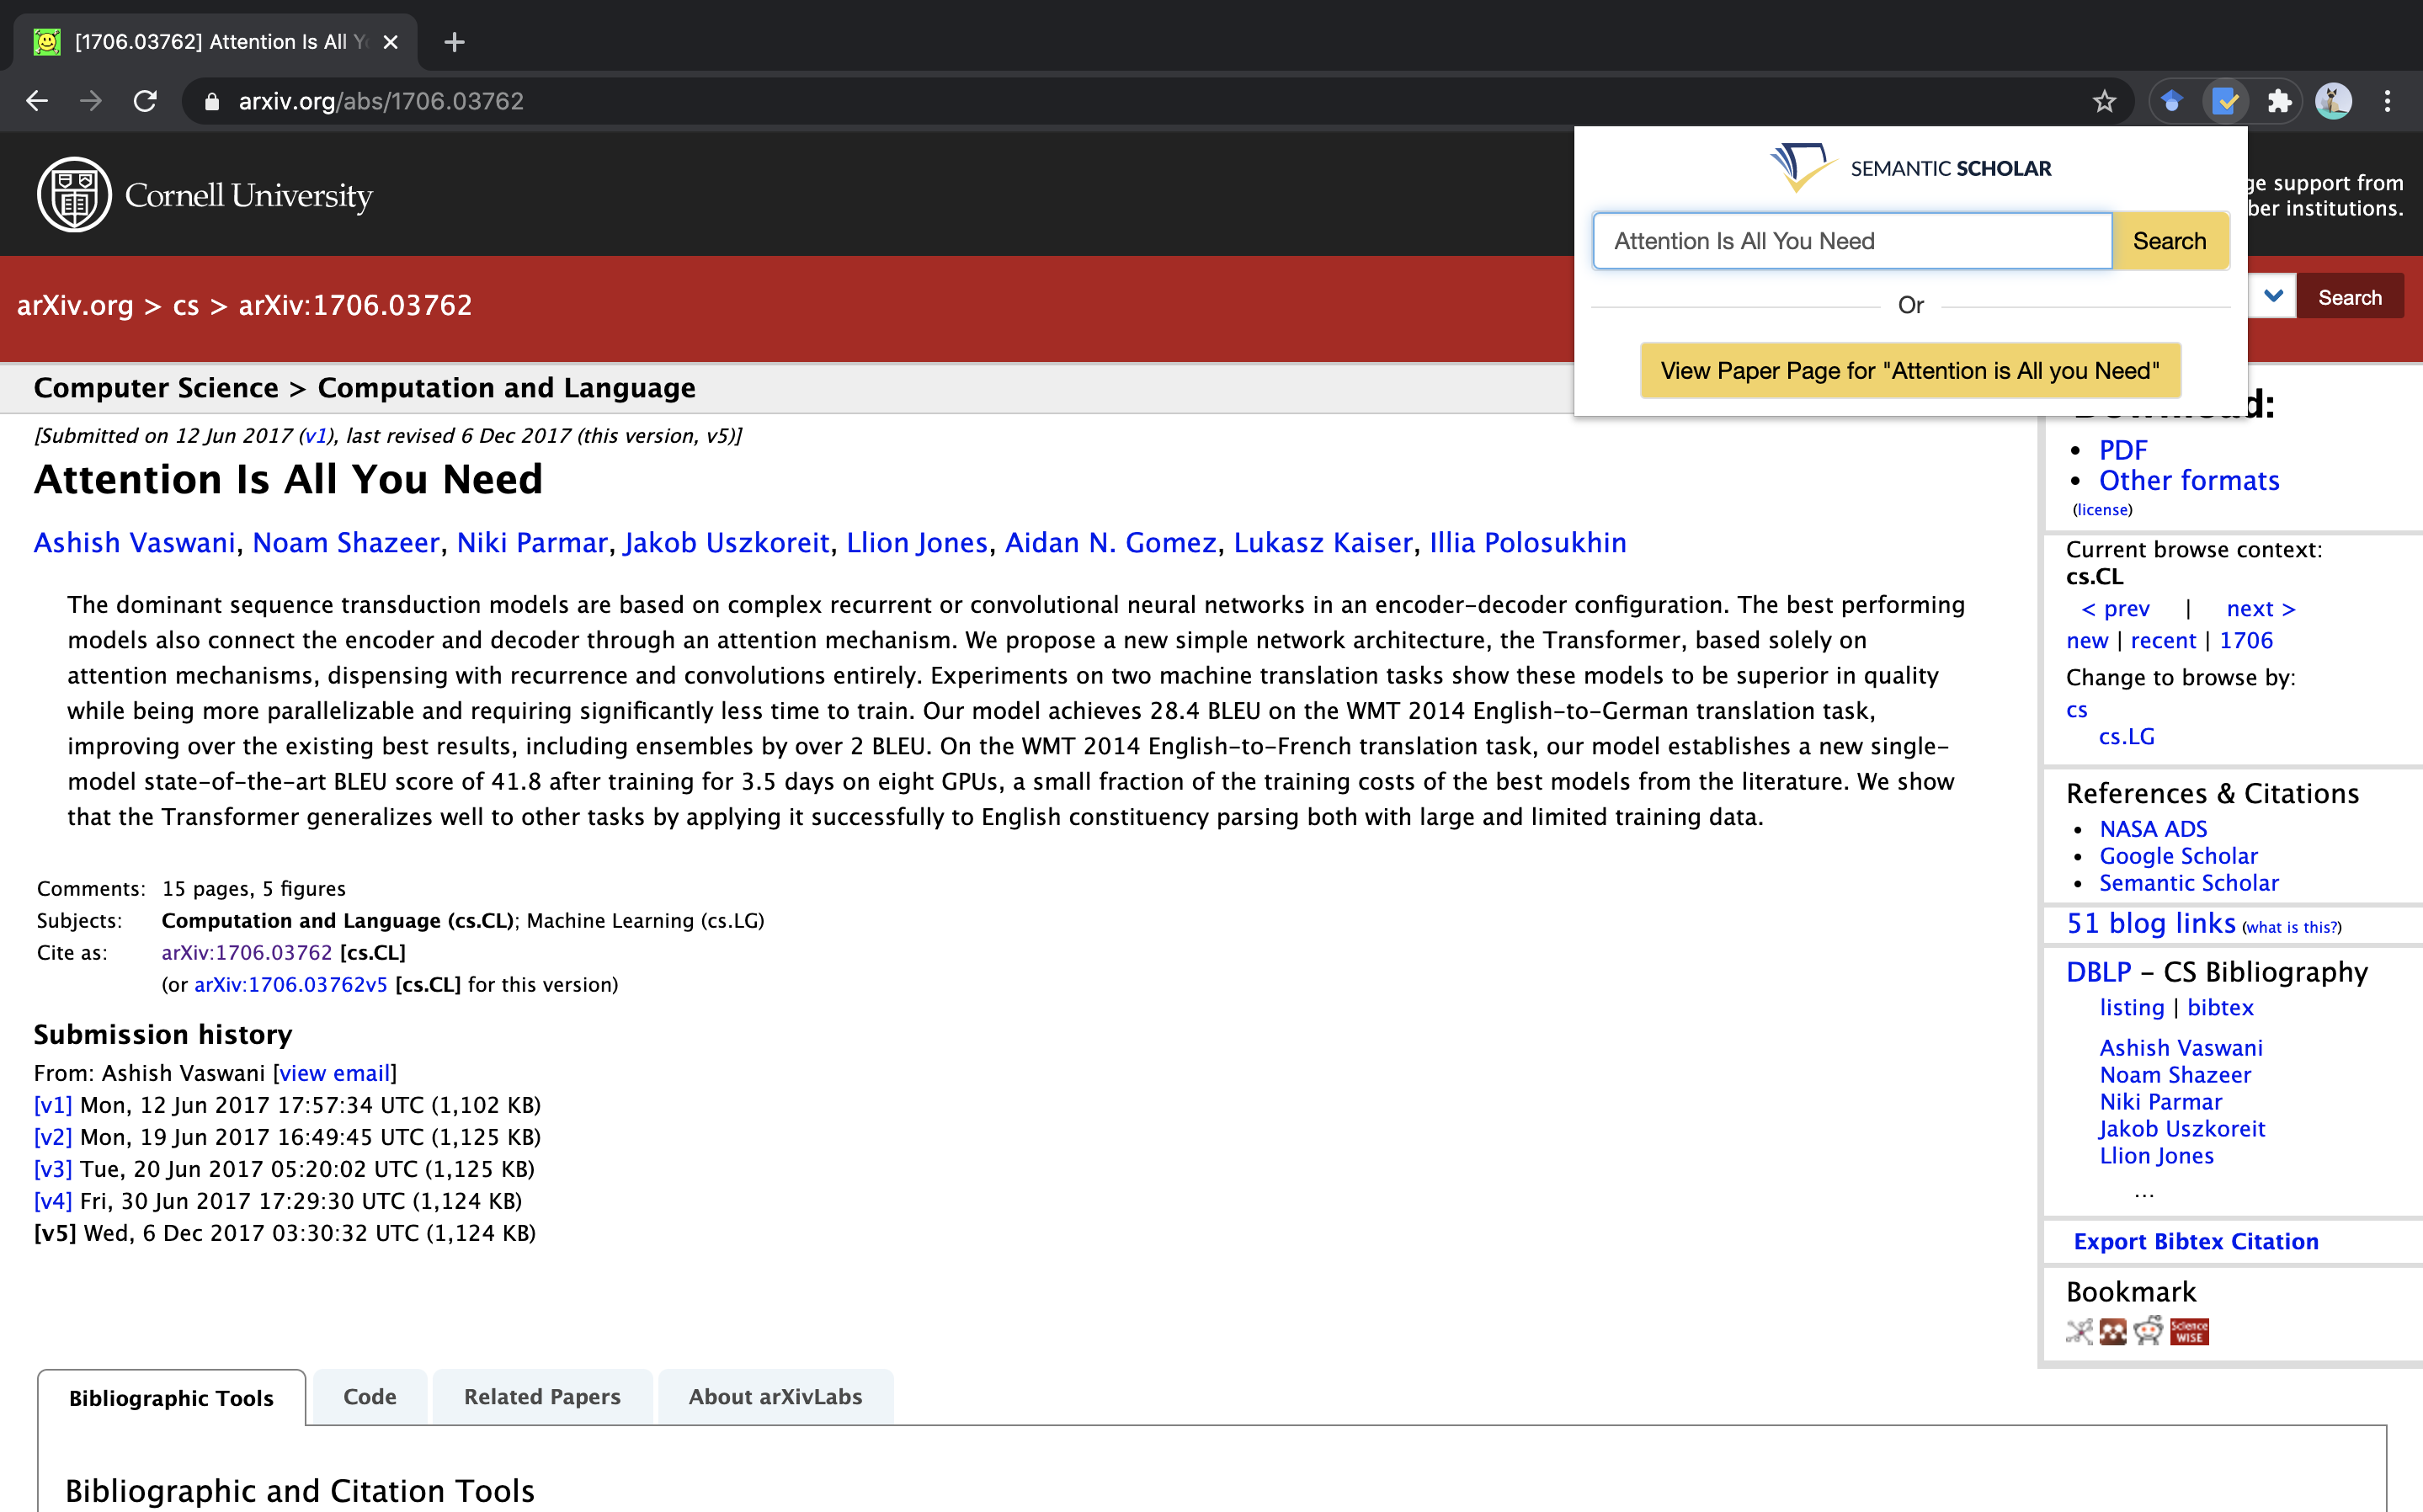
\includegraphics[width=\maxwidth{\textwidth}]{src/images/gg-plugin.png}
    \caption{Chrome(Browser) Plugin For Google Scholar}
    \label{figure\arabic{figurecounter}}
\end{figure}
\refstepcounter{figurecounter}
\begin{figure}[h]
    \centering
    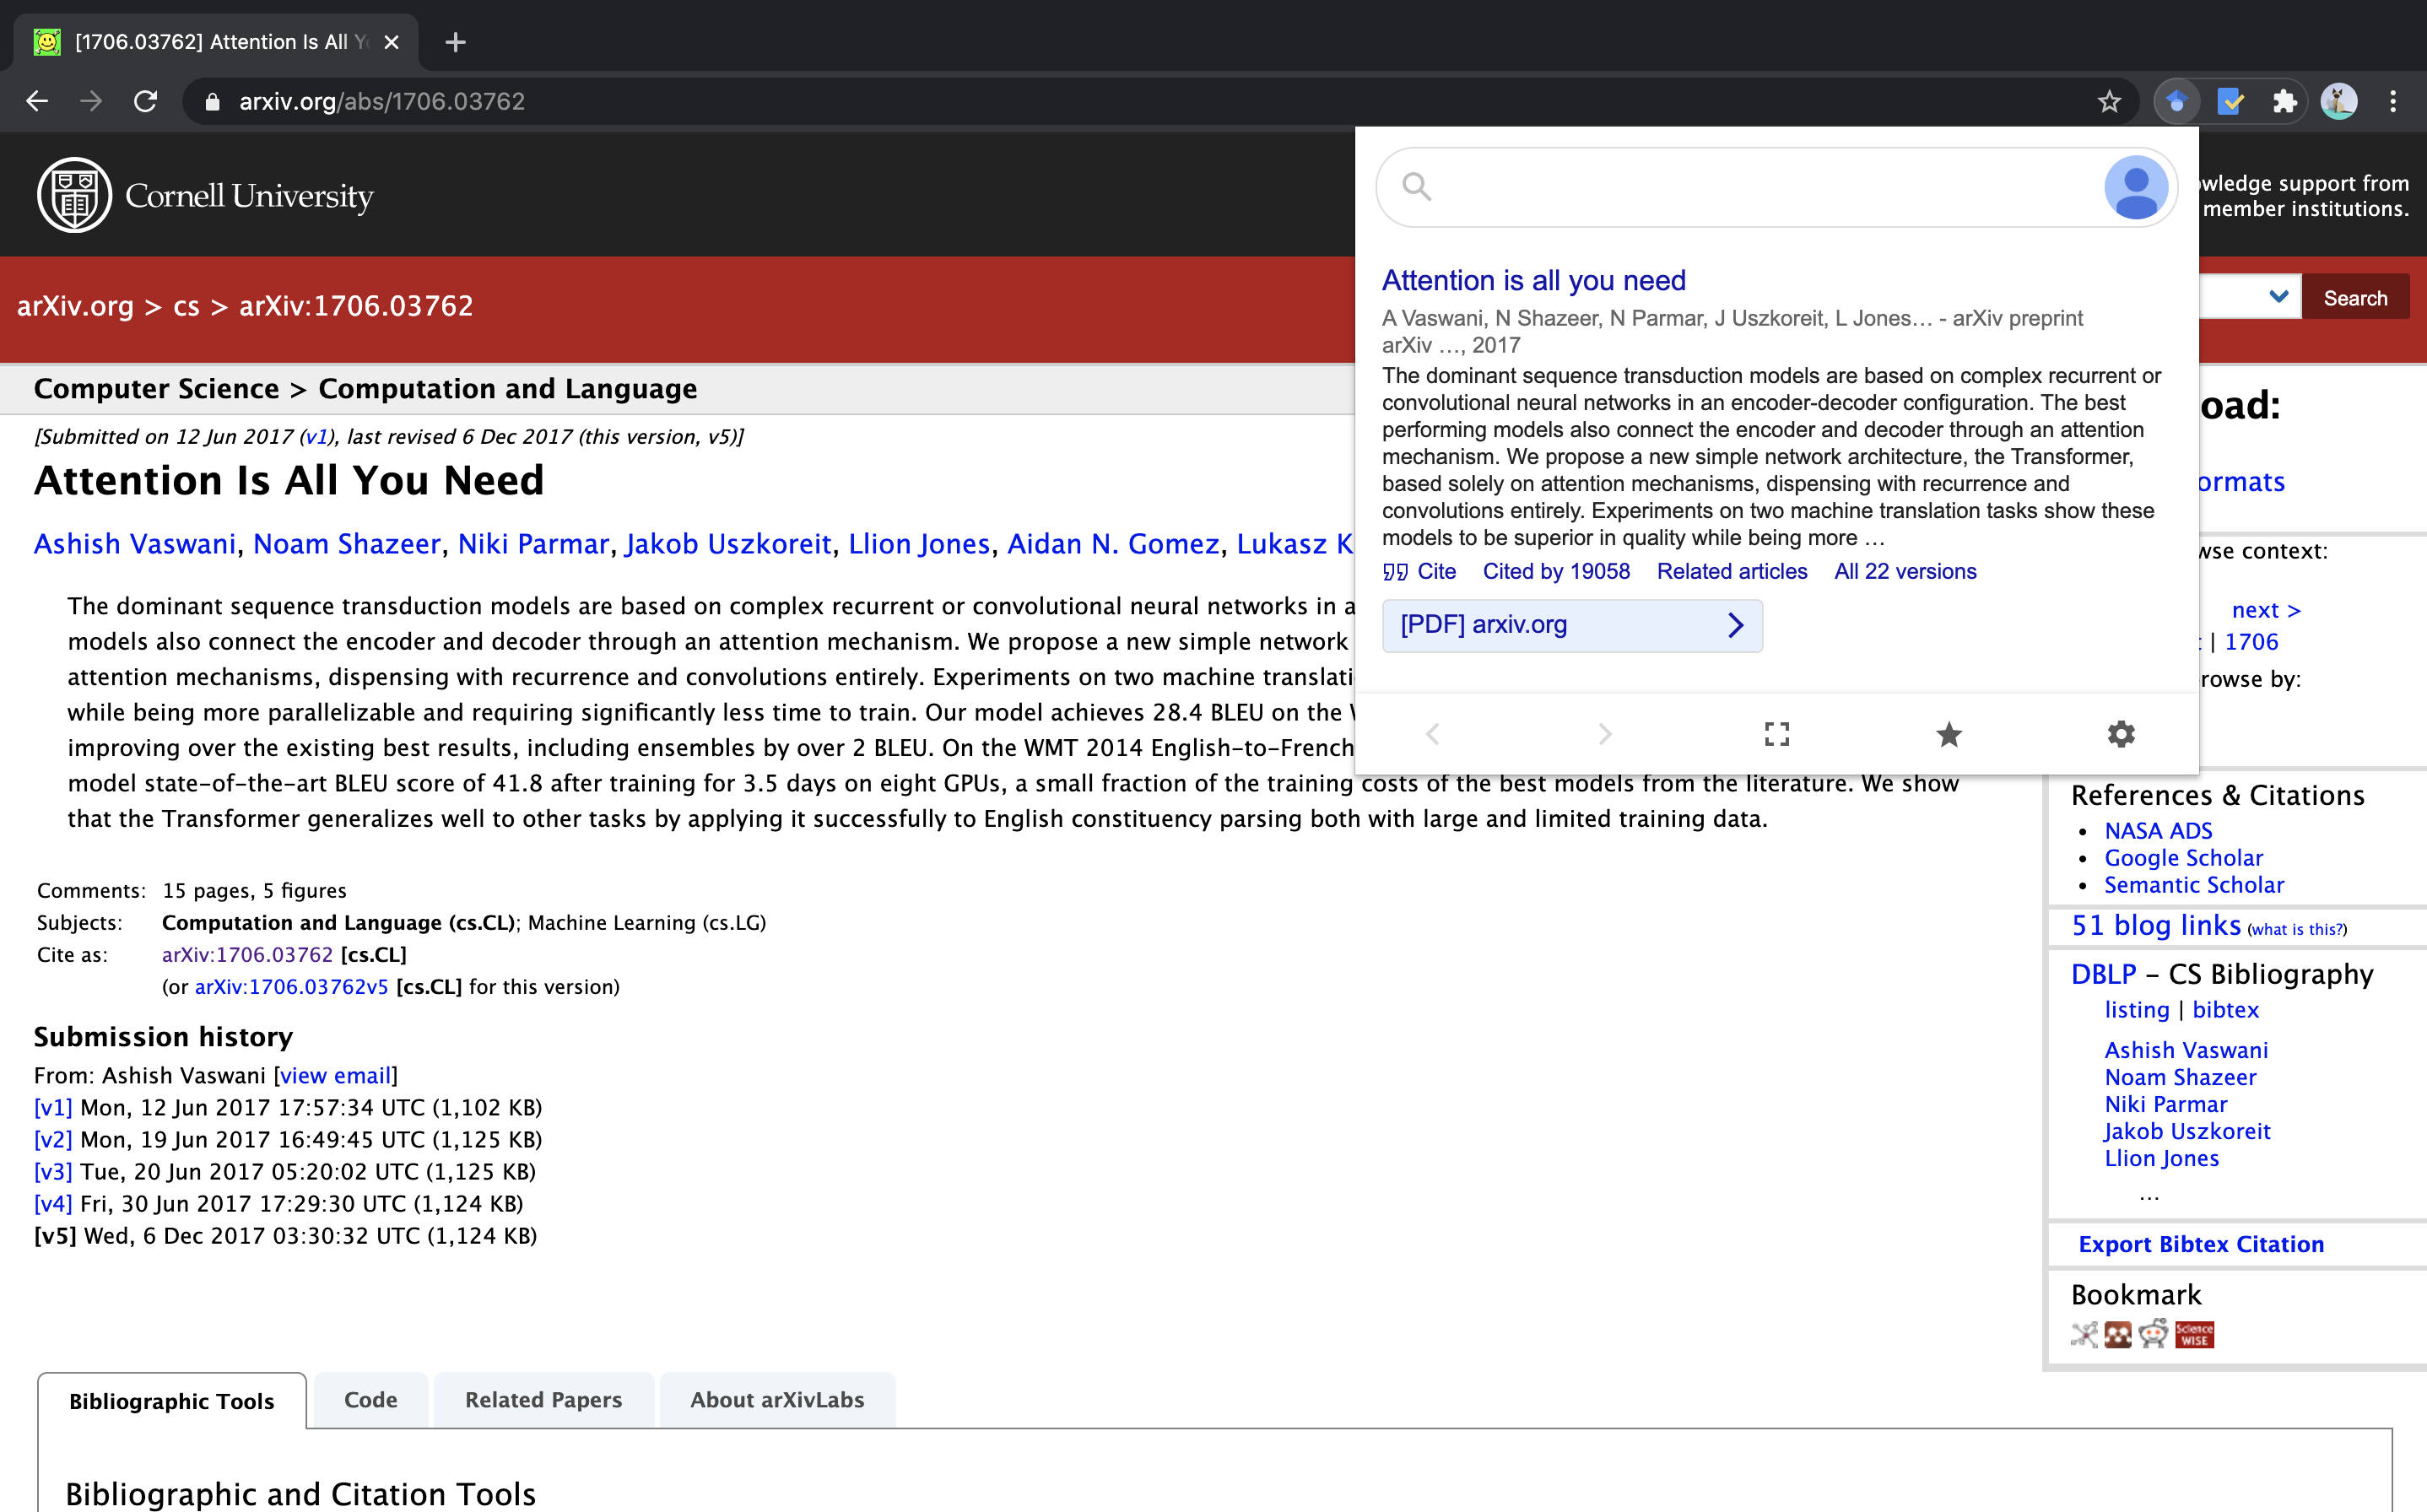
\includegraphics[width=\maxwidth{\textwidth}]{src/images/ss-plugin.png}
    \caption{Chrome(Browser) Plugin For Semantic Scholar}
    \label{figure\arabic{figurecounter}}
\end{figure}
\refstepcounter{figurecounter}
Many scientific literature search engines also offer features such as forward citation search, but these features are not always accessible outside the website of the search engine. 
Google Scholar and Semantic Scholar provide browser extensions to help the researchers get more context on a research document as seen from Figure \ref{figure5} and Figure \ref{figure6}. 
These extensions lead back to the search engine's proprietary websites access more information surrounding the research. 
They also miss out on many essential aspects of research documents such as tables in the research when surfacing relevant information about the document. 
They also do not provide information within the browser when the researcher is reading an article online. 
\pagebreak
\subsection{No Access To More Fine Grained Information Such as Tables When Reading Research}
With the recent growth in Machine Learning publications, new platforms such as PapersWithCode\footnote{https://paperswithcode.com} and 
sotabench\footnote{https://sotabench.com/} help compare State-of-the-art(SOTA) methods from various research papers and link source code 
to many SOTA ML techniques. 

Many research papers compare methods from other research papers and such information is not directly accessible to the
researcher when reading a research article online. Even though these platforms 
host parsed information from raw research, there is no way to intelligently access that information when reading a research paper online. 
This results in researcher spending valuable time finding the cited comparisons.

\section{Proposed Approach And Overview}
This dissertation focuses on the solutions developed to tackle the missing characteristics described in Section \ref{section:intro:missing_traits}. 

Section \ref{relatedwork:background} provides some preliminary background on inverted index based search engines, open-source search engines and state-of-the-art machine learning techniques.
Section \ref{relatedwork:acad-search-engine} discusses the different studies conducted about academic search engines; Section \ref{relatedwork:acad-lit-mining} discusses the different techniques used for mining academic literature; Section \ref{relatedwork:table-type} will discuss previous research to pertaining to classification of tables. 

Section \ref{method} provides an overview of the proposed solutions i.e. a search engine over CS ArXiv and a browser extension to augment research at time of reading 

Section \ref{sci-genie-core} discusses the core components of the search engine and the chrome extension; Section \ref{table_classification}
discusses the problem/application/experiments for table of comparison classification task.
% Section \ref{sci-genie-extension} discusses the packaged solution which leverages the search engine and the table classification methods mentioned in  
% Section \ref{sci-genie-core},Section \ref{table_classification} to help bring context relevant information when reading research articles. 

Finally, Section \ref{conclusion} will provide some insight into future work applicable to the information augmentation/search for academic literature. 